% $Id$
\section{Bending Beam under Uniform Load}
\label{BEAM CHAP}
\sectionauthor{Jannine Eisenmann}{}

Given is a two-dimension bending beam which is fixed in all directions
at the left end and free at the other, see \fig{BEAM FIG 1}. Furthermore the beam is loaded
with a uniform load $p$.

\begin{figure}
% \centerline{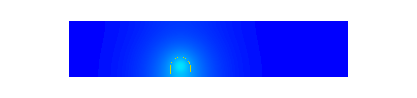
\includegraphics[width=\figwidth]{DiffusionRes1}}
\caption{Loaded Beam.}
\label{BEAM FIG 1}
\end{figure}



For emphasizing the displacement this picture is drawn (uebertrieben),
cause since we use the linear theory otherwise no displacements would
be visible. 
There are two ways of solving this problem: on the one hand one can
use the differential equation for the deformed neutral fibre of the
beam. This classical differential equation is based on several simplifying
assumptions concerning the statics and kinematics of the problem.
However the results are known to be highly accurate at least for slender
beams with length to hight ratios $> 10$. Alternatively, in connection
with finite element based differential equation toolkits one may simply
consider the beam as a special case of a 2D or 3D elastic continuum
problem and solve the stress equilibrium equations combined with Hooke's
law for the specific boundary conditions of a beam. Both cases assume
isotropic and linear elastic material properties.

The beam equation is easily solved analytically. The analytical solutions
can be used for benchmarkung finite element solutions. In section
1.2 we formluate a finite element code for general isotropic elasticity
problems including thin and deep beams under arbitrary loading conditiond
in 2D or 3D. 


\section{2-dimensional}
As the stress equilibrium equation is a partial differential equation
(PDE), we choose to use Finley to solve it, since Finley is a finite
element kernel library, that has been incorporated as a differential
equation solver into the python based numerical toolkit called escript.
We divided the beam into ten square elements of the size 1x1. Each
element consists of 8 nodes, which leads to a quadratic interpolation
of the model point displacements \\

The key ingredients is \textbf{Hooks Law}. We use Hooks Law because
we are dealing with \textbf{linear elastic material} \textbf{behaviour}.
We have \\


$\sigma_{ik}=2G\left(\varepsilon_{ik}+\frac{\nu}{1-2\nu}\cdot e\cdot\delta_{ik}\right)$\hfill{}(1)\\
where the engineering strain$\varepsilon_{ik}$is defined as:

$\varepsilon_{ik}=\frac{1}{2}\cdot\left(u_{k,i}+u_{i,k}\right)$\hfill{}(2)\\


with

\begin{enumerate}
\item e= Volume strain = $\varepsilon_{kk}$
\item $\delta_{ik}$= Kronecker symbol
\end{enumerate}
Inserting equation (2) in (1) (and with further mathematical conversions)
leads to the following partial differential equation :\\


$\sigma_{ij}=\left[\mu\left(\delta_{ik}\delta_{jl}+\delta_{il}\delta_{jk}\right)+\lambda\left(\delta_{ij}\delta_{kl}\right)\right]u_{k,l}$\\


For tension equilibrium we require:\\


$\sigma_{ij,j}=0$\\


which leads to the following expression:\\


\[
\left(\left[\mu\left(\delta_{ik}\delta_{jl}+\delta_{il}\delta_{jk}\right)+\lambda\left(\delta_{ij}\delta_{kl}\right)\right]u_{k,l}\right)_{,j}=0\]


with the natural boundary condition:

\[
n_{j}\sigma_{ij}=-p_{i}\]
\\
$p_{i}$ representing a uniform load on top of the beam.

A Dirichlet Boundary condition is assumed on the left end of the beam
for which no displacements can occure.\\
\\
\includegraphics[%
  width=0.60\linewidth,bb = 0 0 200 100, draft, type=eps]{/home/jeannine/sandbox/report/draws/dir_cond_beam.eps}\\
This is described in the code with the setting a mask for the left
end and setting values to that mask:

\begin{python}
q = xNodes{[}0{]}.whereZero(){*}{[}1.0,1.0{]}

r = Vector({[}0.0, 0.0{]}, where = nodes)
\end{python}
The Finley template PDE reads:\\


\[
-(A_{ijkl}u_{k,l})_{,j}-(B_{ijk}u_{k})_{,j}+C_{ikl}u_{k,l}+D_{ik}u_{k}=-X_{ij,j}+Y_{i}\]
\\
with the natural boundary condition:

\[
n_{j}(A_{ijkl}u_{k,l}+B_{ijkl}u_{k})+d_{ik}u_{k}=n_{j}X_{ij}+y_{i}on\Gamma_{i}^{D}\]


Yields by comparing the coefficients :

\begin{enumerate}
\item $A_{ijkl}$= $\left[\mu\left(\delta_{ik}\delta_{ij}+\delta_{jl}\delta_{il}\right)+\lambda\left(\delta_{ij}\delta_{kl}\right)\right]$
\item $y_{i}$= $-p_{i}$
\item $u_{k}$= displacement $u$
\end{enumerate}
$B_{ijk,}=C_{ikl}=D_{ik}=X_{ij}=Y_{i}=d_{ik}=0$\\


Where 0 in the last line is taken as a scalar, vector or tensor, depending
on what the belonging coefficient is.

These equations are the base for the \textbf{Finley Script}:

\begin{python}
from ESyS import {*}
import Finley



\#mu lamda

def mu (E, nu): \#= shear modul G

     return E/(2{*}(1+nu))

def lamda (E, nu):

     return (nu{*}E)/((1-2{*}nu){*}(1+nu))



def main()

     \#material, beam PROPERTIES

     L = 10.0         \#length of beam {[}m{]}

     h = 1            \#height of beam {[}m{]}

     p = 1            \#outer uniform load {[}kN/m{]}

     E0 = 210000      \#Young's modulus {[}kN/m\textasciicircum{}2{]}

     nu = 0.4         \#Poisson ratio {[}-{]}



     print \char`\"{}L=\char`\"{}, L

     print \char`\"{}h=\char`\"{}, h

     print \char`\"{}p=\char`\"{}, p

     print \char`\"{}E=\char`\"{}, E0

     print \char`\"{}nu=Poisson =\char`\"{}, nu

     print \char`\"{}mu=\char`\"{}, mu (E0,nu)

     print \char`\"{}lamda=\char`\"{}, lamda (E0,nu) 



     \#SET MESH for FE

     mesh= Finley.Rectangle(n0=10 ,n1=1 ,order=2, l0=L, l1=h)

     nodes = mesh.Nodes()

     xNodes = nodes.getX()

     elements = mesh.Elements()

     faceElements = mesh.FaceElements()

     xFaceElements = faceElements.getX()



     \#DISPLACEMENT boundary

     q = xNodes{[}0{]}.whereZero(){*}{[}1.,1.0{]}    \#setting the                                           mask for r

     r = Vector({[}0.0, 0.0{]}, where = nodes) \#fixed end



     \#STRESS boundary

     ymask = xFaceElements{[}1{]}.whereEqualTo(h)

     y = Vector({[}0, -p{]}, where = faceElements)

     y = y{*}ymask



     \#Finley coeff.

     A = Tensor4(0, where = elements)

     for i in range (2) :

        for j in range (2) :

           A{[}i,i,j,j{]}+= lamda (E0,nu)

           A{[}j,i,j,i{]}+= mu (E0,nu)

           A{[}j,i,i,j{]}+= mu (E0,nu)



     M,b = mesh.assemble(A=A, B=B, q=q,         

     y=y,r=r,type=CSR,num\_equations=2)

     u= M.iterative(b, tolerance=1e-8,iter\_max=50000,

     iterative\_method=PCG)

     print \char`\"{}u{[}0{]}=\char`\"{},u{[}0{]}

     print \char`\"{}u{[}1{]}=\char`\"{},u{[}1{]}

main()
\end{python}
The finer the mesh the more exact is the solution. E.g. a 20x2 mesh
is more exact than a 10x1 mesh. 

